% mainfile: ../../../../master.tex
\subsection{DNA and RNA quantification with NanoDrop Spectrophotometer}
% The part of the label after the colon must match the file name. Otherwise,
% conditional compilation based on task labels does NOT work.
\label{task:20180201_cj5}
\tags{dna,rna,lab,qnt}
\authors{cj}
%\files{}
%\persons{}

\subsubsection{DNA quantification with NanoDrop}

Purity ratios are important indicators of sample quality. Pure DNA is supposed to have a 260/280 ratio of 1.8. Here the 260/280 ratio is 2.53 (cf. figure \ref{fig:CJ20180201_DNA}) which is a lot higher than expected which may indicated the presence of protein or other contaminant (here we did not use phenol, so I doubt that the contaminant is phenol). The expected values of the ratio 260/230 are between 1.8 to 2.0 for pure nucleic acids. Here the value is 1.53 which is a lot lower.

\begin{figure}[H] % position of the figure 
    \centering
    \caption{Screen capture of the NanoDrop analysis for the extracted DNA}
    \label{fig:CJ20180201_DNA}
    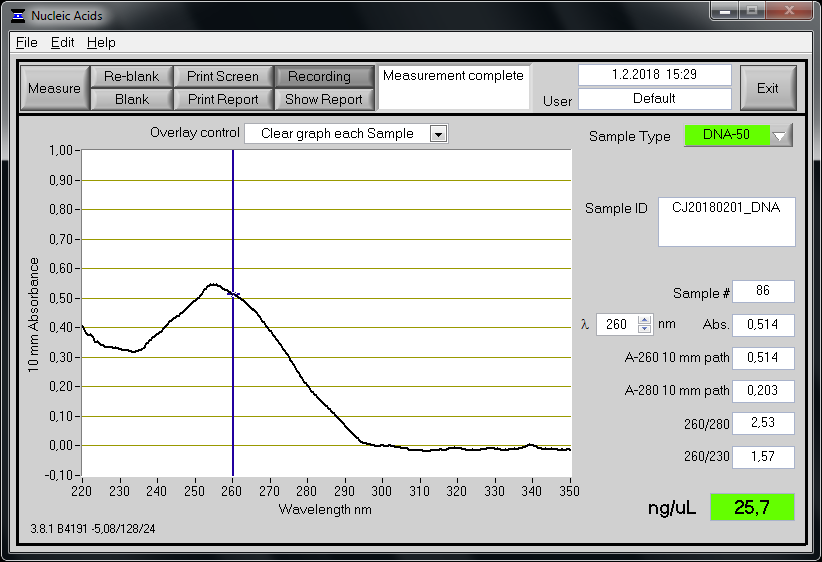
\includegraphics[width=\textwidth]{graphics/screenshots/CJ20180201_DNA.png}
\end{figure}

So here, the DNA extracted with the MasterPure\texttrademark kit is not very pure. This could be explained by my inexperience as it is the very first time I use this kit. \sidenote{Mia Cerfonteyn was able to obtain DNA with purity ratio values matching the expected values.} In any case, the best indicator of the DNA qyality is its functionality in the downstream application of interest: I must try to amplify this DNA by PCR.

\subsubsection{RNA quantification with NanoDrop}

Pure RNA is supposed to have a 260/280 ratio of 2 but I obtained a value of 1.79 which suggests the presence of contaminants.

\begin{figure}[H] % position of the figure 
    \centering
    \caption{Screen capture of the NanoDrop analysis for the extracted RNA}
    \label{fig:CJ20180201_RNA}
    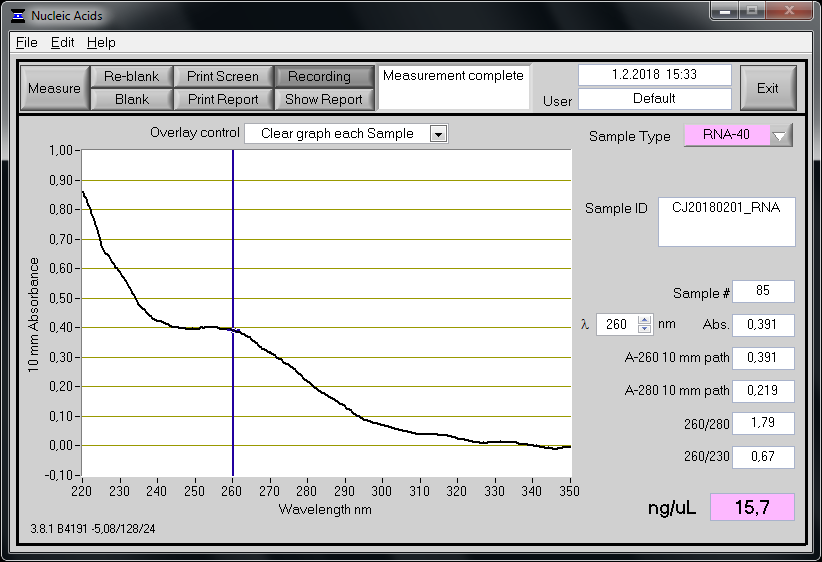
\includegraphics[width=\textwidth]{graphics/screenshots/CJ20180201_RNA.png}
\end{figure}

The conclusion is for the RNA is the same as for the DNA. It is not pure ...





